\documentclass[a4paper,12pt,oneside]{book}

%-------------------------------Start of the Preamble------------------------------------------------
\usepackage[english]{babel}
\usepackage{blindtext}
\usepackage{hyperref}
\usepackage{hyperref} %packagr for hyperlinks
\usepackage{fancyhdr} %use of package fancy header
\usepackage{titlesec} %use of package for section title formatting
\usepackage[most]{tcolorbox} %use of package tcolorbox for colorful textbox
\usepackage{marginnote} %use of package marginnote for notes in margin
%use of packgage watermark for pages
%\usepackage{draftwatermark}
%\SetWatermarkText{
\includegraphics{logo}}
\usepackage[scale=2,opacity=0.1,angle=0]{background}
\usepackage{xcolor} %use of newcommand for keywords color
\usepackage{graphicx} %package for inserting pictures
\usepackage{color,soul} %package for highlighting
\newcommand{\head}[1]{\textnormal{\textbf{#1}}} %new command for table

\usepackage{subfiles}

\usepackage{listings}
\usepackage{color}
\usepackage{tikz}

\definecolor{dkgreen}{rgb}{0,0.6,0}
\definecolor{gray}{rgb}{0.5,0.5,0.5}
\definecolor{mauve}{rgb}{0.58,0,0.82}

\lstset{frame=tb,
	language=C,
	aboveskip=3mm,
	belowskip=3mm,
	showstringspaces=false,
	columns=flexible,
	basicstyle={\small\ttfamily},
	numbers=none,
	numberstyle=\tiny\color{gray},
	keywordstyle=\color{blue},
	commentstyle=\color{dkgreen},
	stringstyle=\color{mauve},
	breaklines=true,
	breakatwhitespace=true,
	tabsize=3
}

\hypersetup{
	colorlinks=true,
	linkcolor=black,
	filecolor=red,
	urlcolor= cyan,
}
\urlstyle{same}

\fancyhf{}
\setlength\headheight{26pt}

\lhead{\rightmark}
\rhead{
\includegraphics[width=1cm]{Images/logo.png}}

\fancyfoot[RE, RO]{\thepage}
\fancyfoot[CE, CO]{\href{http://www.e-yantra.org}{www.e-yantra.org}}
\pagestyle{fancy}

\titleformat{\chapter}
{\Large\bfseries} % format
{}                % label
{0pt}             % sep
{\huge}           % before-code


\tcbset{colback=cyan!5!white,colframe=cyan!75!black,halign title = flush center}
\newtcolorbox{mybox}[1]{colback=cyan!5!white,
	colframe=cyan!75!black,fonttitle=\bfseries,
	title=\textbf{\Large{#1}}}

\backgroundsetup{
	contents={
\includegraphics{Images/logo}}
}

\newcommand{\keyword}[1]{\textcolor{red}{\textbf{#1}}}

\newcommand{\ExternalLink}{%
	\tikz[x=1.2ex, y=1.2ex, baseline=-0.05ex]{% 
		\begin{scope}[x=1ex, y=1ex]
			\clip (-0.1,-0.1) 
			--++ (-0, 1.2) 
			--++ (0.6, 0) 
			--++ (0, -0.6) 
			--++ (0.6, 0) 
			--++ (0, -1);
			\path[draw, 
			line width = 0.5, 
			rounded corners=0.5] 
			(0,0) rectangle (1,1);
		\end{scope}
		\path[draw, line width = 0.5] (0.5, 0.5) 
		-- (1, 1);
		\path[draw, line width = 0.5] (0.6, 1) 
		-- (1, 1) -- (1, 0.6);
	}
}

%----------------------End of the Preamble---------------------------------------

\begin{document}
	
	%---------------------Title Page------------------------------------------------
	\begin{titlepage}
		\raggedright
		{\Large eYSIP2017\\[1cm]}
		{\Huge\scshape Formation Control of Multiple Swarm Robots \\[.1in]}
		\vfill
		\begin{flushright}
			{\large Chirag Shah \\}
			{\large Om Singh \\}
			{\large \textbf{Mentors:}Abhinav Sarkar \\}
			{\large Avinash Kumar Dubey\\}
			{\large Duration of Internship: $ 22/05/2017-07/07/2017 $ \\}
		\end{flushright}
		
		{\itshape 2017, e-Yantra Publication}
	\end{titlepage}
	%-------------------------------------------------------------------------------
	
	\tableofcontents
	\pagebreak
	
	\chapter[Formation Control of Multiple Swarm Robots]{Formation Control of Multiple Swarm Robots}
	\subfile{abstract}
		
	\section{Project Overview}
	
		The objective of the project is to control multiple robots simultaneously to form any desired shapes. The shapes can be predefined: like the shapes of letters, or can be drawn on the screen. The robots will then attempt to form the shapes.
		
		The robots used are Spark V from Nex Robotics. The robots are controlled using a python script running on a laptop (master). The robots are localized using ArUco markers placed on the robots. The markers provide the coordinates and the orientation of each of the robots. OpenCV libraries are used along with python for the detection of ArUco markers.
		
		XBee radio modules are used for the communication between the laptop and the robots.
		
		The laptop can individually communicate with each robot. It sends the robot's position and orientation to the robot along with the desired position of that robot. The robot then moves towards the required position using a Go-to-Goal PID controller running on the robot.	Thus multiple robots are directed to the required positions to form a desired shape.\\
		
		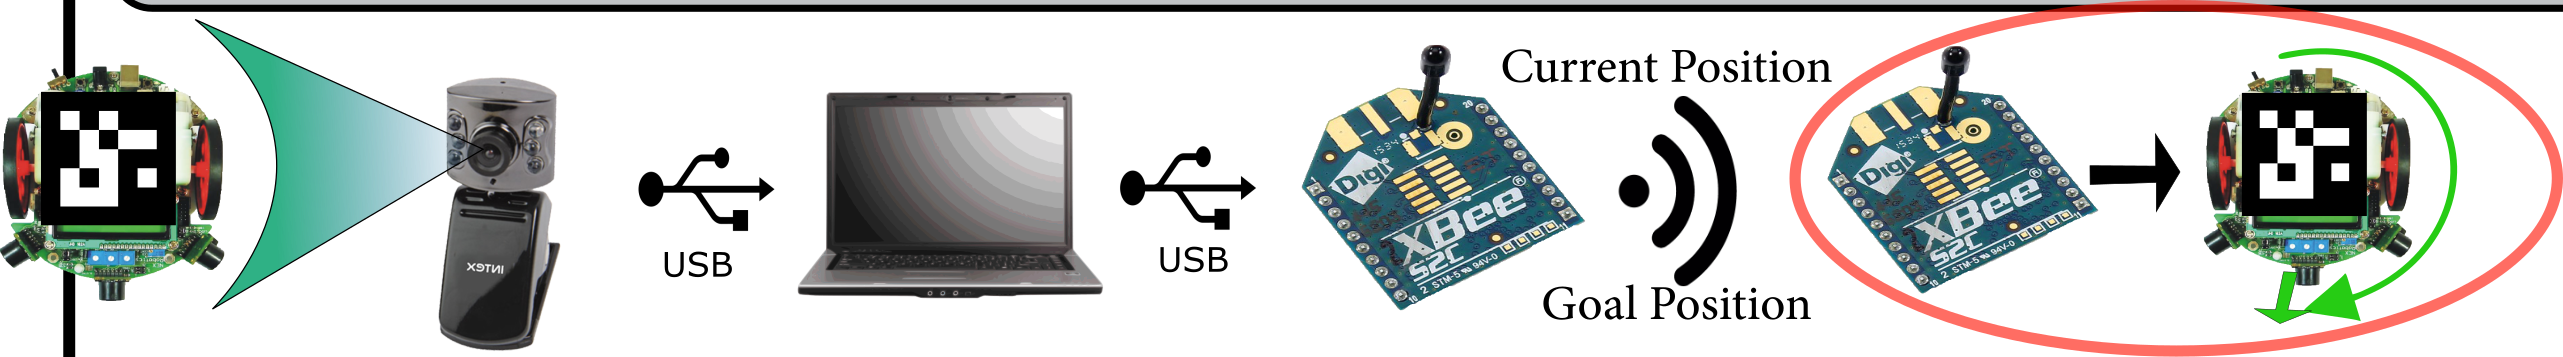
\includegraphics[scale = .2]{Images/flow.png}
		
	\section{Completion status}
	\begin{itemize}
		\item Aruco markers are reliably used for obtaining the position and orientation of Spark V robots
		\item Go-To-Goal is implemented using a PID controller on the Spark V robot
		\item The robots can form most letters 
		\item A desired formation can be obtained given by drawing it on the screen
	\end{itemize}
		
	\subfile{HardwareandSoftware/hardwareandsoftware}
	\subfile{XBee/XBeeConfiguration}
	\subfile{AVR/AVR}
	\subfile{Python/Python}
	
	\chapter[Project Tag]{Use and Demo}
	
	\section{Challanges}
	\begin{itemize}
		\item When using the on board IR sensors, they would detect any obstacle successfully, but they would also be triggered by the IR from the other robots in the arena even from a considerable (3-4 feet). It was concluded that the only way to use the onboard sensors was to make hardware changes like adding a transistor for switching the sensors.
		\item If the XBees were kept in AT mode so that the data of every robot is received by each robot, the robot was not able to handle a large amount of data (of more then 3-4 robots). The robot would go into some undefined behavior and had to be reset. This was suspected to be because having a long interrupt function for communication on the robot and the buffer becoming full with a large amount of data.\\
		This was an issue for having collision avoidance on the robot. This might be solved by having better communication algorithms (like circular buffers) on the robot.
	\end{itemize}
		
	\section{Bug report}
	With the current python script, occasionally the error "index list out of range" occurs during runtime.\\
	Positions of the goal points sometimes are very close together. Averaging of points in the list may not be appropriate for some shapes.\\
	Shapes need to be drawn in a single stroke.\\
	
	\section{Future Work}
	This is potentially a very powerful swarm robotics system as we can obtain the state of each robot with respect to a global co-ordinate system.\\
	The robot can know the state of all the robots. Hence collision avoidance and neighboring robot detection can be moved to the robot. Since the robot knows the position of every robot, algorithms for different swarm behaviors can be developed.\\
	Complex swarm behaviors can be obtained by implementing the algorithms for inter-robot communication.\\
	Algorithm for drawing shapes and for goal point allocation for robots can be improved.\\
	
	
	\begin{thebibliography}{li}
		\bibitem{OpenCV docs}
		OpenCV docs
		\href{http://docs.opencv.org/3.1.0/d5/dae/tutorial_aruco_detection.html}{\ExternalLink}
		
		\bibitem{Aruco detection blog}
		Aruco detection blog
		\href{http://www.philipzucker.com/aruco-in-opencv/}{\ExternalLink}

		\bibitem{OpenCV docs - ArUco detection}
		OpenCV docs - ArUco detection
		\href{http://docs.opencv.org/3.1.0/d5/dae/tutorial_aruco_detection.html}{\ExternalLink}
		
		\bibitem{Control of Mobile Robots}
		Courcera-Control of Mobile Robots
		\href{https://www.coursera.org/learn/mobile-robot}{\ExternalLink}
		
		\bibitem{}
		XBee library for python
		\href{https://pypi.python.org/pypi/XBee}{\ExternalLink}
		
		\bibitem{}
		Wikipedia - Distance martix
		\href{https://en.wikipedia.org/wiki/Distance_matrix}{\ExternalLink}
		
		\bibitem{}
		OpenCV - User Interface
		\href{http://docs.opencv.org/2.4/modules/highgui/doc/user_interface.html}{\ExternalLink}
		
		\bibitem{}
		Sparkfun XBee Guide
		\href{https://learn.sparkfun.com/tutorials/exploring-xbees-and-xctu}{\ExternalLink}
		
		\bibitem{}
		API mode guide
		\href{https://dzone.com/articles/xbee-zigbee-complaint}{\ExternalLink}
		
	\end{thebibliography}
	
\end{document}

